\section{Evaluation}
\subsection{CIFAR-10 Experiments}
\begin{frame}{CIFAR-10 Experiments}
\framesubtitle{A General Image Classification Task}
  \vspace{-1em}
  \CifarDatasetSlide
\end{frame}
\note{
- Only a short refresher \\
}


\begin{frame}{CIFAR-10 Experiments}
\framesubtitle{Performance Characteristics and Insights, CIFAR-10}
  \vspace{-2em}
  \begin{figure}
    \centering\hspace*{-2em}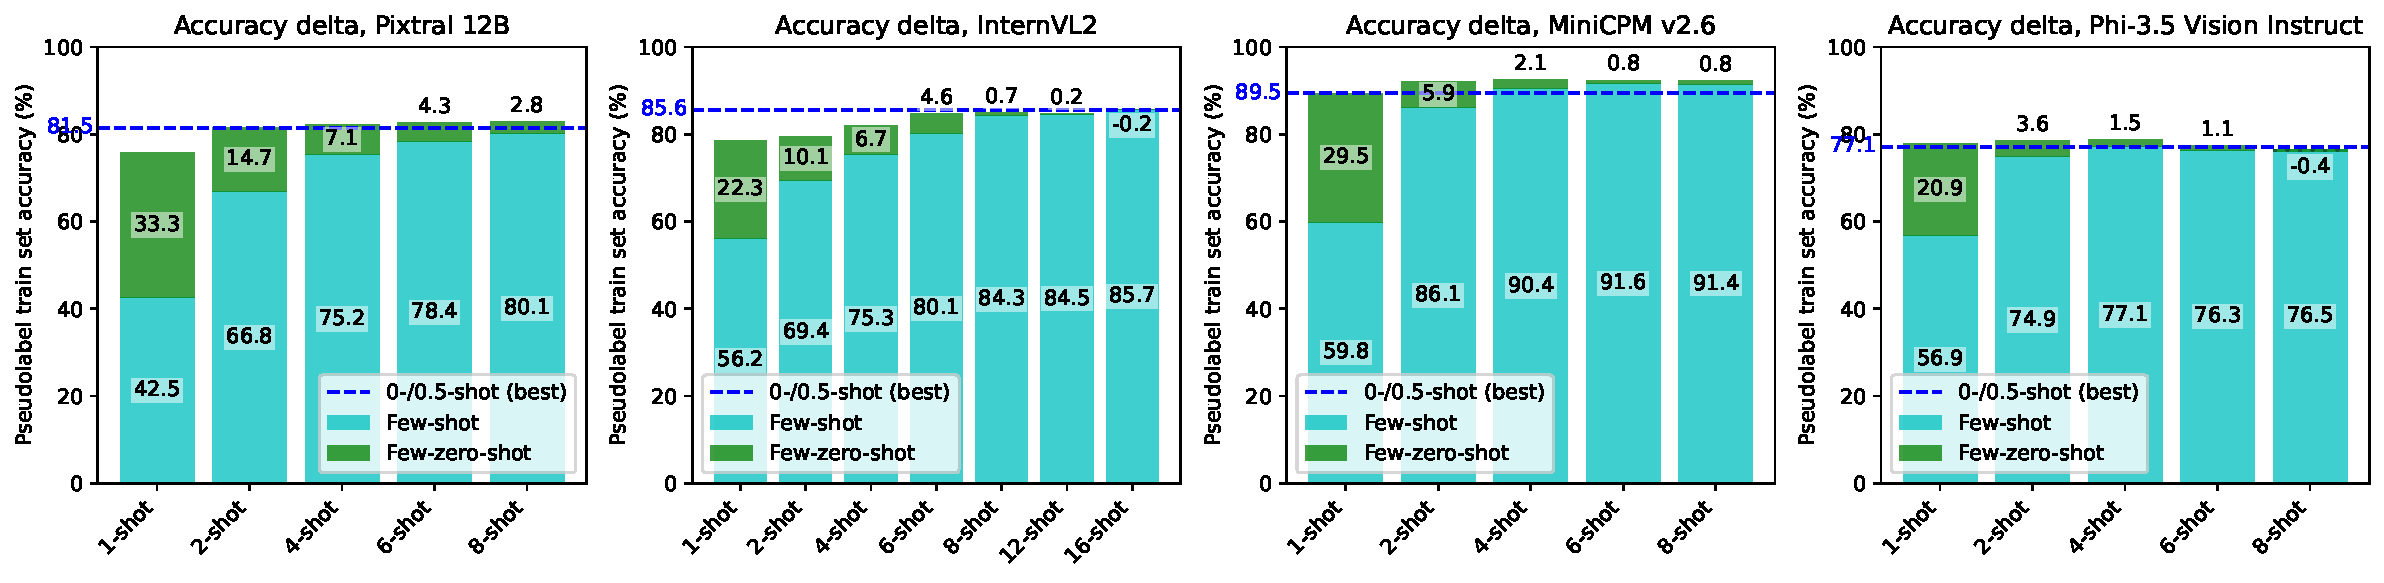
\includegraphics[width=1.1\linewidth]{figures/cifar_accuracy_delta_few_zero_shot_over_few_shot.pdf}
    \vspace{-1.6em}
    \caption{\centering Visualization of VLM performance in few-shot experiments \textcolor{lightblue}{without} and \textcolor{darkgreen}{with textual prompt} with \textcolor{darkblue}{zero-shot-best baseline}; the differences are shown}
  \end{figure}
  \vspace{-1.6em}
  \begin{itemize}
    \setlength{\itemsep}{0em}
    \item Providing \textcolor{darkgreen}{textual prompt} significantly helps low-shot model understand task, constraints
    \item Performance generally peaks at 4-8 examples, still close to \textcolor{darkblue}{zero-shot best}
  \end{itemize}
\end{frame}
\note{
- Without prompting, model generates predictions not in class list, leading to a large number of invalid predictions \\
- With enough examples, model `learns' the class list, supporting the idea that the model `recognizes' the task and its constraints rather than `learn' it \\
}


% \subsection{Downstream Model Analysis}
\begin{frame}{Downstream Model Analysis}
\framesubtitle{Performance Characteristics and Insights, CIFAR-10}
  \vspace{-2em}
  \begin{figure}
    \centering\hspace*{-2em}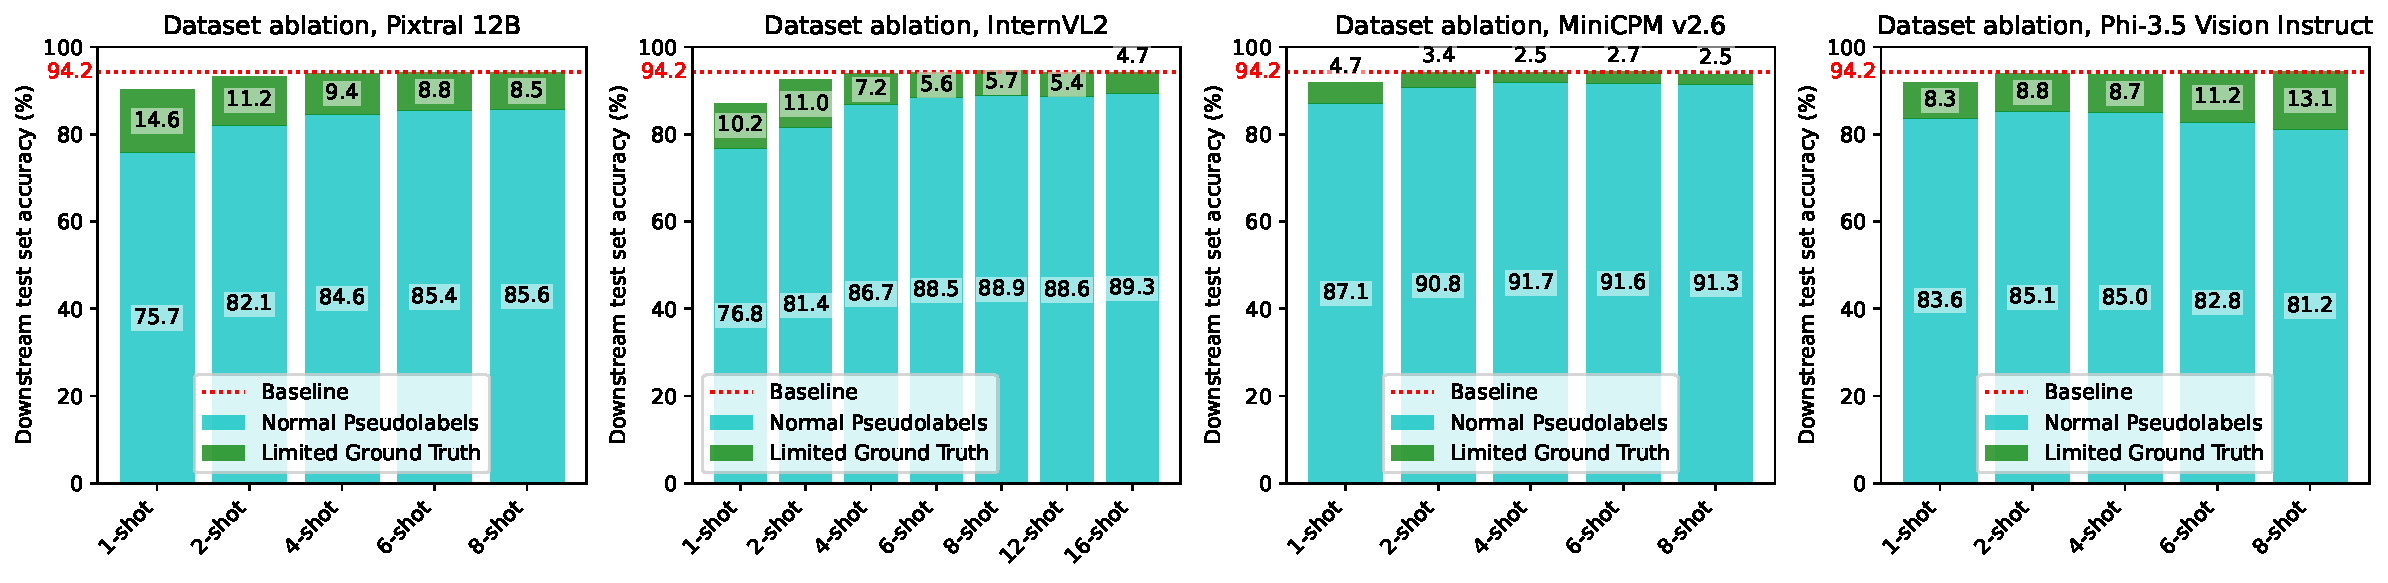
\includegraphics[width=1.1\linewidth]{figures/cifar_downstream_model_accuracy_delta_limited_gt_over_normal.pdf}
    \vspace{-1.6em}
    \caption{\centering Visualization of downstream model performance trained on few-shot \textcolor{lightblue}{pseudolabels} and \textcolor{darkgreen}{limited ground truth labels} with \textcolor{darkred}{ground truth model baseline}; the differences are shown}
  \end{figure}
  \vspace{-1.6em}
  \begin{itemize}
    \setlength{\itemsep}{0em}
    \item Performance \textcolor{darkgreen}{difference to limited ground truth} due to label noise in \textcolor{lightblue}{pseudolabels} 
    \item \emph{Weak dependence} of downstream performance on \emph{example count}
    \item Generally outperformed VLMs that generated the \textcolor{lightblue}{pseudolabels}
  \end{itemize}
\end{frame}
\note{
- Downstream models consistently outperformed VLMs due to ImageNet pre-training and focus on pattern recognition \\
- Label quality proved more important than dataset size in training. In few-shot experiments, 33\% of the labels were invalid and hence is equivalent to a reduction in dataset size by 33\% \\
- However, the performance was still acceptable, with only a minor drop in performance compared to a model trained on ground truth labels with the same invalid labels taken out. Practicaly utility -- can use imperfect data \\
- Downstream model performance has weak dependence on example count, meaning both dataset size and number of shots
- Downstream models consistently outperformed VLMs due to ImageNet pre-training and focus on pattern recognition \\
}


\subsection{Seven-Point Checklist Dermatology Experiments}
\begin{frame}{Dermatology Experiments}
\framesubtitle{Experiment Setup and Evaluation Framework}
  \vspace{-1em}
  \DermPtDatasetSlide{\DermPtFigureOne}
\end{frame}
\note{
- Only a short refresher \\
- We have two tasks: one that tries to predict the diagnosis directly from the images, and another that predicts each of the seven checklist features from the images \\
- Idea: Maybe the model finds it difficult to predict the condition directly, so maybe it is better to predict the features first?
}


% \begin{frame}{Dermatology Experiments}
% \framesubtitle{Key Findings}
%   \vspace{-1em}
%   \begin{columns}[T]
%     \column{\customcolumnwidth}
%       \textbf{Performance Patterns}
%       \begin{itemize}
%         \item Models performed near random-guess accuracy
%         \item Addition of clinical images as well as reasoning requirements often degraded performance
%         \item Domain-tuned model struggled with poor instruction following, failing most experiments
%       \end{itemize}
%     \column{\customcolumnwidth}
%       \textbf{Key Challenges}
%       \begin{itemize}
%         \item Limited pre-training knowledge
%         \item Multi-modal integration issues
%         \item Performance degradation with:
%         \begin{itemize}
%           \item Increased examples
%           \item Added reasoning requirements
%           \item Multiple image modalities (addition of clinical images)
%         \end{itemize}
%       \end{itemize}
%   \end{columns}
% \end{frame}
% \note{
% - Most models near random-guess accuracy, indicating fundamental limitations of VLMs for this task \\
% - The domain-specific Biomedical Multimodal Model struggled, and this is likely because the fine-tuning caused regressions in the instruction-following capabilities of the model. This is somewhat of a known issue, and goes along the lines of catastrophic forgetting -- but this is something that a few-shot or zero-shot transferred model may not suffer from \\
% - It seems we are at the limits of what and how much can be provided as inputs to the model, as well as the knowledge of the model itself \\
% }



\begin{frame}{Dermatology Experiments}
\framesubtitle{Performance in Direct Condition Diagnosis}
  \vspace{-3em}
  \begin{figure}
    \centering\hspace*{-2em}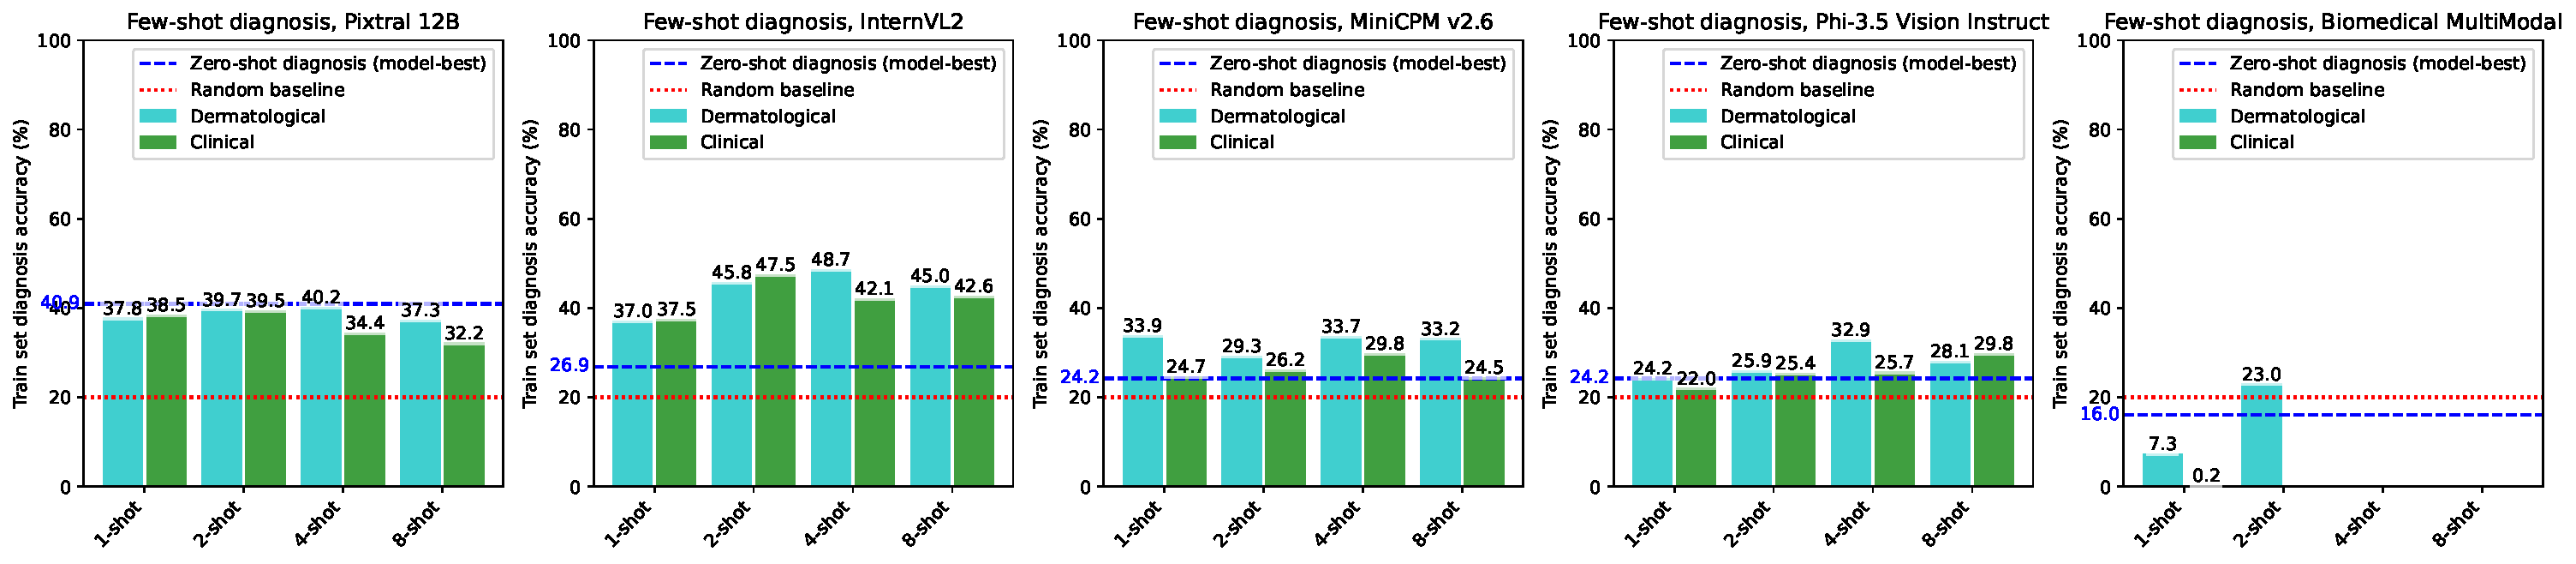
\includegraphics[width=1.1\linewidth]{figures/derm7pt_few_shot_diagnosis_clinical_over_derm.pdf}
    \vspace{-1.6em}
    \caption{\centering Visualization of VLM performance \textcolor{lightblue}{without} and \textcolor{darkgreen}{with clinical images} in few-shot diagnosis experiments}
  \end{figure}
  \vspace{-1em}
  Some models perform around \textcolor{darkred}{random-guess accuracy}
  \vspace{-0.2em}
  \begin{itemize}
    \setlength{\itemsep}{0em}
    \item Some improvement over \textcolor{darkblue}{best zero-shot performance baseline}
    \item \emph{Diminishing returns} with examples
    \item Addition of \textcolor{darkgreen}{clinical images} generally degrades performance
    \item General failure of domain-fine-tuned model
  \end{itemize}
\end{frame}
\note{
- Direct diagnosis showed some promise with few-shot learning \\
- Few-shot performance generally peaks at 2-4 examples \\
- Only best zero-shot performance results shown here, but reasoning requirements generally decreased model performance \\
- Only Pixtral 12B had zero-shot performance notable better than random guessing, but the other models caught up with few-shot prompting \\
- The domain-specific Biomedical Multimodal Model struggled, and this is likely because the fine-tuning caused regressions in the instruction-following capabilities of the model. This is somewhat of a known issue, and goes along the lines of catastrophic forgetting -- but this is something that a few-shot or zero-shot transferred model may not suffer from \\
}


\begin{frame}{Dermatology Experiments}
\framesubtitle{Performance in Structured Feature Understanding}
  \vspace{-3em}
  \begin{figure}
    \centering\hspace*{-2em}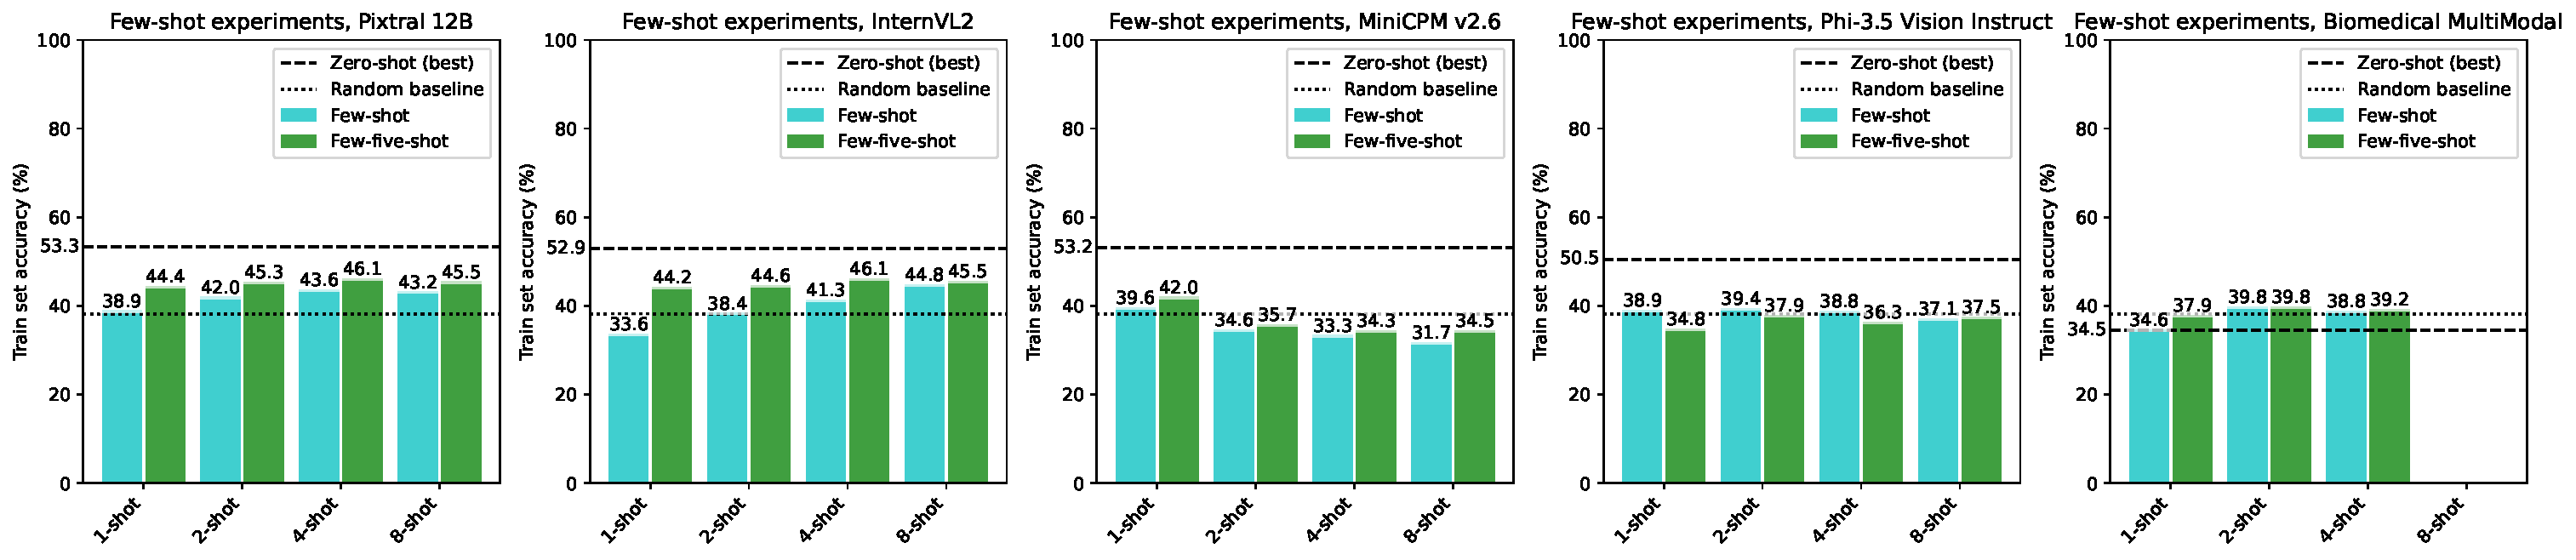
\includegraphics[width=1.1\linewidth]{figures/derm7pt_few_five_over_few_shot_structured_derm.pdf}
    \vspace{-1.6em}
    \caption{\centering Visualization of VLM performance \textcolor{lightblue}{without} and \textcolor{darkgreen}{with additional task information} in few-shot structured feature understanding}
  \end{figure}
  \vspace{-1em}
  Models perform around \textcolor{darkred}{random-guess accuracy}
  \vspace{-0.2em}
  \begin{itemize}
    \setlength{\itemsep}{0em}
    \item General drop from \textcolor{darkblue}{best zero-shot performance baseline}
    \item \emph{Diminishing returns} with more examples
    \item Providing \textcolor{darkgreen}{additional task information} produces minor improvements
  \end{itemize}
\end{frame}
\note{
- Few-shot performance generally peaks at 2-4 examples \\
- Domain-fine-tuned model appears to have recognized the task this time, but is well in random-guessing territory like the other models \\
}


% \begin{frame}{Implications}
% \framesubtitle{What did we learn from the experiments?}
%   \vspace{-1em}
%   \begin{columns}[T]
%     \column{\customcolumnwidth}
%       \textbf{Key Insights}
%       \begin{itemize}
%         \item Pre-training knowledge crucial:
%           \begin{itemize}
%             \item Poor performance on specialized tasks
%             \item Transferability to specialized domains not guaranteed
%           \end{itemize}
%         \item Architectural considerations:
%           \begin{itemize}
%             \item Model size \(\nRightarrow\) performance
%             \item Multi-modal integration challenges exist
%           \end{itemize}
%         \item Downstream learning resilient
%         \item Few-shot transfer is closer to task \emph{recognition} than task learning
%       \end{itemize}
%     \column{\customcolumnwidth}
%       \textbf{Future Directions} -- specialized training strategies needed:
%       \begin{itemize}
%         \item for domain-transferable pre-training
%         \item to improve multi-modal integration
%       \end{itemize}
%       \textbf{Practical Considerations}
%       \begin{itemize}
%         \item Prefer simpler prompting strategies
%         \item Consider resource-performance trade-offs
%         \item Models pre-trained on multi-image, multi-turn conversation -- better
%       \end{itemize}
%   \end{columns}
% \end{frame}
% \note{
% - Context length and memory limitations restricted few-shot experiments to limited examples and constrained larger models \\
% - Observed trends already show limited/degraded performance scaling with higher number of examples \\
% - Poor performance on specialized domains suggests models rely more on pre-trained priors than learning new capabilities \\
% - Promising research directions include investigating domain-specific pre-training strategies \\
% - Formulate task-specific evaluation metrics to see where or what part of the task cause issues, and work with prompting strategies to improve performance \\
% - Each kind of image is a different modality in the dermatology case. The model may not know how to look at both image which are two forms of the same thing, and reason and understand the relationship between the two. The integration of the two modalities is a challenge. How do you look at to forms of the same thing and reason about the relationship between the two? \\
% }


% The compute analysis is too detail-heavy to show in a presentation
% \subsection{Compute Analysis}
% \begin{frame}{Compute Analysis}
% \framesubtitle{Analysis of Memory and Processing Time}
%   \vspace{-1em}
%   \begin{columns}[T]
%     \column{\customcolumnwidth}
%       \textbf{Memory Usage Patterns}
%       \begin{itemize}
%         \item Model-dependent example scaling:
%         \vspace{-1.2em}
%         \begin{itemize}
%           \item Pixtral 12B: \emph{Super-linear}
%           \item InternVL2, Phi-3.5: \emph{Linear}
%           \item MiniCPM: \emph{Near-constant} (perceiver-resampler)
%         \end{itemize}
%         \item Double image inputs (dermatology experiments): 1-1.75x increase (compared to single image inputs)
%         \item \emph{Less} than the expected \emph{quadratic} scaling for pure transformers~\footfullciteieee{Vaswani2017}
%       \end{itemize}
%     \column{\customcolumnwidth}
%       \textbf{Processing Time Impact}
%       \begin{itemize}
%         \item Significant increase with examples (compared to zero-shot):
%         \vspace{-1.2em}
%         \begin{itemize}
%           \item 2 examples: \(\sim\)10x longer
%           \item 4 examples: \(\sim\)20x longer
%           \item 8 examples: 30-50x longer
%         \end{itemize}
%         \item Reasoning requirements: 10-35\% longer (compared to zero-shot)
%         \item Double image inputs (dermatology experiments): 1.5-2.5x longer (compared to single image inputs)
%       \end{itemize}
%   \end{columns}
% \end{frame}
% \note{
% - Memory usage patterns vary significantly between model architectures \\
% - MiniCPM's perceiver-resampler architecture enables near-constant memory usage regardless of examples \\
% - Clinical images (additional images) increase memory usage by 1-1.75x \\
% - Processing time increases dramatically with number of examples used \\
% - Adding reasoning requirements (e.g., chain-of-thought) increases processing time by 10-35\% due to the generation of more output tokens \\
% - Clinical images take 1.5-2.5x longer to process due to increased number of images and complexity \\
% - These patterns align with theoretical expectations for optimized transformer architectures, and are lower than the expected quadratic scaling \\
% }


% \begin{frame}{Compute Analysis}
% \framesubtitle{Practical Implications}
%   \vspace{-1em}
%   \begin{columns}[T]
%     \column{\customcolumnwidth}
%       \textbf{Resource-Performance Trade-offs} -- Diminishing returns with examples:
%       \begin{itemize}
%         \item Performance peaks at \(\sim\)4 examples
%         \item Resource costs can grow super-linearly
%       \end{itemize}
%     \column{\customcolumnwidth}
%       \textbf{Recommendations} -- Optimizing for practical deployment:
%       \begin{itemize}
%         \item Zero-shot or 1-2 shots with prompting
%         \item Avoid reasoning requirements (unless the task calls for it)
%         \item Single-image-per-turn processing when possible
%       \end{itemize}
%   \end{columns}
%   \vspace{1em}
%   \textbf{Architecture and model pre-training considerations:}
%     \begin{itemize}
%       \item Perceiver-resampler based models more efficient
%       \item Larger model size \(\nRightarrow\) better performance
%     \end{itemize}
% \end{frame}
% \note{
% - Resource costs grow much faster than performance improvements with additional examples \\
% - Perceiver-resampler architectures (like in MiniCPM) show better memory efficiency \\
% - However, there may be a trade-off between resource efficiency and model performance \\
% - Zero-shot or low-shot (1-2 examples) provides best balance of performance vs. resources \\
% - Avoiding reasoning requirements saves significant processing time without major performance loss \\
% - Why does reasoning not work? The tasks we chose are not reasoning-heavy tasks, but rather test visual recognition and grounding capabilities. Ungrounded reasoning cannot improve the recognition and grounding capabilties of the model \\
% - Multi-image processing (e.g., clinical + dermoscopic) significantly impacts resources \\
% - Architecture choice crucial for scaling to larger datasets or more complex tasks \\
% - These findings help inform practical deployment strategies for VLMs in real applications \\
% }